\clearpage
\subsection{premi/client/presentation}
\begin{figure}[H]
\begin{center}
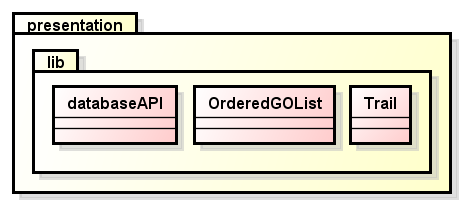
\includegraphics[scale=0.90]{img/diapkg/presentation.png}
\caption{Diagramma del package premi/client/presentation}
\end{center}
\end{figure}


%-------  diagramma della classe%
\subsubsection{premi/client/presentation/lib/databaseAPI}
\begin{figure}[H]
\begin{center}
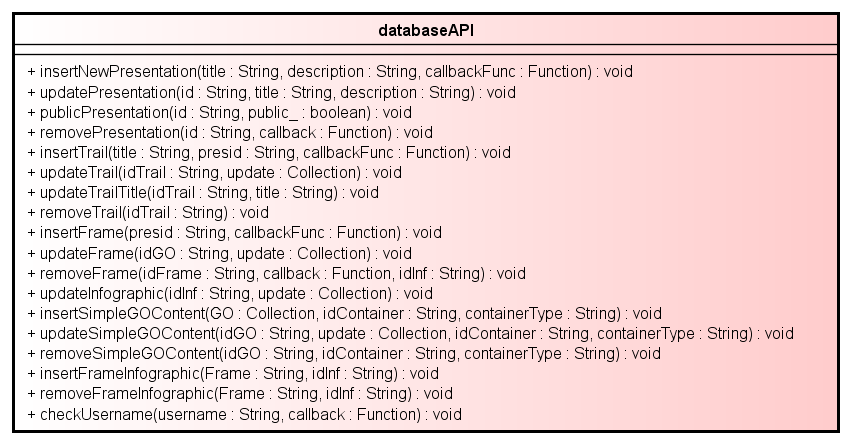
\includegraphics[scale=0.55]{img/diacla/databaseAPI.png}
\caption{Diagramma della classe premi/client/presentation/lib/databaseAPI}
\end{center}
\end{figure}


\begin{description}
%-------  descrizione della classe%
\item[Descrizione] \hfill
	Classe di metodi statici che permette al client di interfacciarsi ai metodi corrispondenti del server
	
	
%-------  lista dei metodi%	
\item[Metodi] \hfill

	% -- inizio metodo -- %
	\begin{description}
		\item[\textbf{\color{blue}+ insertNewPresentation(title : String, description : String, callbackFunc : Function) : void			}] \hfill
			Permette l'inserimento di una nuova presentazione all'interno del database
			
		\begin{description}
			% -- lista argomenti del metodo -- %
			\item[Argomenti] \hfill
				\begin{itemize}
				
					\item \textbf{title : String			} \hfill
					Titolo della nuova presentazione
					\item \textbf{description : String			} \hfill
					Descrizione della nuova presentazione
					\item \textbf{callbackFunc : Function			} \hfill
					Funzione di callback$_G$ per la restituzione dell'id della presentazione
					
				\end{itemize}
			% -- note aggiuntive sul metodo -- %
			\item[Note] \hfill
			\begin{itemize}
					\item Chiama il metodo \textit{insertPresentation} pubblicato in \textit{\$meteor}
			\end{itemize}
		\end{description}
	\end{description}
	% -- fine metodo -- %		



	% -- inizio metodo -- %
	\begin{description}
		\item[\textbf{\color{blue}+ updatePresentation(id : String, title : String, description : String) : void			}] \hfill
			Permette l'aggiornamento del titolo e della descrizione di una presentazione dell'utente
			
		\begin{description}
			% -- lista argomenti del metodo -- %
			\item[Argomenti] \hfill
				\begin{itemize}
					\item \textbf{id : String			} \hfill
					Codice identificativo della presentazione da aggiornare
					\item \textbf{title : String			} \hfill
					Nuovo titolo della presentazione
					\item \textbf{description : String			} \hfill
					Nuova descrizione della presentazione
					
				\end{itemize}
			% -- note aggiuntive sul metodo -- %
			\item[Note] \hfill
			\begin{itemize}
					\item Chiama il metodo \textit{editPresentation} pubblicato in \textit{\$meteor}
			\end{itemize}
		\end{description}
	\end{description}
	% -- fine metodo -- %		


	% -- inizio metodo -- %
	\begin{description}
		\item[\textbf{\color{blue}+ publicPresentation(id : String, public\_ : boolean) : void			}] \hfill
			Rende una presentazione pubblica o privata
			
		\begin{description}
			% -- lista argomenti del metodo -- %
			\item[Argomenti] \hfill
				\begin{itemize}
					\item \textbf{id : String			} \hfill
					Codice identificativo della presentazione da aggiornare
					\item \textbf{public\_ : boolean			} \hfill
					Variabile booleana: se \textit{true} la presentazione verrà resa pubblica, se \textit{false} verrà resa privata
					
				\end{itemize}
			% -- note aggiuntive sul metodo -- %
			\item[Note] \hfill
			\begin{itemize}
					\item Chiama il metodo \textit{publicPresentation} pubblicato in \textit{\$meteor}
			\end{itemize}
		\end{description}
	\end{description}
	% -- fine metodo -- %		


	% -- inizio metodo -- %
	\begin{description}
		\item[\textbf{\color{blue}+ removePresentation(id : String, callback : Function) : void			}] \hfill
			Permette la rimozione di una presentazione dell'utente dal database
			
		\begin{description}
			% -- lista argomenti del metodo -- %
			\item[Argomenti] \hfill
				\begin{itemize}
					\item \textbf{id : String			} \hfill
					Codice identificativo della presentazione da rimuovere
					\item \textbf{callbackFunc : Function			} \hfill
					Funzione di callback$_G$ per la restituzione di una conferma dell'avvenuta rimozione della presentazione
					
				\end{itemize}
			% -- note aggiuntive sul metodo -- %
			\item[Note] \hfill
			\begin{itemize}
					\item Chiama il metodo \textit{removePresentation} pubblicato in \textit{\$meteor}
			\end{itemize}
		\end{description}
	\end{description}
	% -- fine metodo -- %		



	% -- inizio metodo -- %
	\begin{description}
		\item[\textbf{\color{blue}+ insertTrail(title : String, presid : String, callbackFunc : Function) : void			}] \hfill
			Permette l'inserimento di un trail all'interno del database
			
		\begin{description}
			% -- lista argomenti del metodo -- %
			\item[Argomenti] \hfill
				\begin{itemize}
					\item \textbf{title : String			} \hfill
					Titolo del trail da inserire
					\item \textbf{presid : String			} \hfill
					Codice identificativo della presentazione associata al trail
					\item \textbf{callbackFunc : Function			} \hfill
					Funzione di callback$_G$ per la restituzione del codice identificativo del nuovo trail creato
					
				\end{itemize}
			% -- note aggiuntive sul metodo -- %
			\item[Note] \hfill
			\begin{itemize}
					\item Chiama il metodo \textit{insertTrail} pubblicato in \textit{\$meteor}
			\end{itemize}
		\end{description}
	\end{description}
	% -- fine metodo -- %		
	
	% -- inizio metodo -- %
	\begin{description}
		\item[\textbf{\color{blue}+ updateTrail(idTrail : String, update : Collection) : void			}] \hfill
			Permette l'aggiornamento di un trail
			
		\begin{description}
			% -- lista argomenti del metodo -- %
			\item[Argomenti] \hfill
				\begin{itemize}
					\item \textbf{idTrail : String			} \hfill
					Codice identificativo del trail da aggiornare
					\item \textbf{update :  Collection			} \hfill
					Collezione di MongoDB degli attributi aggiornati del trail
					
				\end{itemize}
			% -- note aggiuntive sul metodo -- %
			\item[Note] \hfill
			\begin{itemize}
					\item Chiama il metodo \textit{updateTrail} pubblicato in \textit{\$meteor}
			\end{itemize}
		\end{description}
	\end{description}
	% -- fine metodo -- %	
	
	% -- inizio metodo -- %
	\begin{description}
		\item[\textbf{\color{blue}+ updateTrailTitle(idTrail : String, title : String) : void			}] \hfill
			Permette la modifica del titolo di un trail
			
		\begin{description}
			% -- lista argomenti del metodo -- %
			\item[Argomenti] \hfill
				\begin{itemize}
					\item \textbf{idTrail : String			} \hfill
					Codice identificativo del trail da aggiornare
					\item \textbf{title : String			} \hfill
					Nuovo titolo del trail
					
				\end{itemize}
			% -- note aggiuntive sul metodo -- %
			\item[Note] \hfill
			\begin{itemize}
					\item Chiama il metodo \textit{updateTrailById} pubblicato in \textit{\$meteor}
			\end{itemize}
		\end{description}
	\end{description}
	% -- fine metodo -- %	
	
	% -- inizio metodo -- %
	\begin{description}
		\item[\textbf{\color{blue}+ removeTrail(idTrail : String) : void			}] \hfill
			Permette la rimozione di un trail dal database
			
		\begin{description}
			% -- lista argomenti del metodo -- %
			\item[Argomenti] \hfill
				\begin{itemize}
					\item \textbf{idTrail : String			} \hfill
					Codice identificativo del trail da rimuovere
					
				\end{itemize}
			% -- note aggiuntive sul metodo -- %
			\item[Note] \hfill
			\begin{itemize}
					\item Chiama il metodo \textit{removeTrailById} pubblicato in \textit{\$meteor}
			\end{itemize}
		\end{description}
	\end{description}
	% -- fine metodo -- %	
	
	% -- inizio metodo -- %
	\begin{description}
		\item[\textbf{\color{blue}+ insertFrame(presid : String, callbackFunc : Function) : void			}] \hfill
			Permette l'inserimento di un frame all'interno del database
			
		\begin{description}
			% -- lista argomenti del metodo -- %
			\item[Argomenti] \hfill
				\begin{itemize}
					\item \textbf{presid : String			} \hfill
					Codice identificativo della presentazione associata al nuovo frame
					\item \textbf{callbackFunc : Function			} \hfill
					Funzione di callback$_G$ per la restituzione del codice identificativo del nuovo frame
					
				\end{itemize}
			% -- note aggiuntive sul metodo -- %
			\item[Note] \hfill
			\begin{itemize}
					\item Chiama il metodo \textit{insertFrameByIdPres} pubblicato in \textit{\$meteor}
			\end{itemize}
		\end{description}
	\end{description}
	% -- fine metodo -- %	
	
	% -- inizio metodo -- %
	\begin{description}
		\item[\textbf{\color{blue}+ updateFrame(idGO : String, update : Collection) : void			}] \hfill
			Permette l'aggiornamento di un frame all'interno del database
			
		\begin{description}
			% -- lista argomenti del metodo -- %
			\item[Argomenti] \hfill
				\begin{itemize}
					\item \textbf{idGO : String			} \hfill
					Codice identificativo del frame da aggiornare
					\item \textbf{update : Collection			} \hfill
					Collezione di MongoDB di attributi aggiornati
					
				\end{itemize}
			% -- note aggiuntive sul metodo -- %
			\item[Note] \hfill
			\begin{itemize}
					\item Chiama il metodo \textit{editFrameById} pubblicato in \textit{\$meteor}
			\end{itemize}
		\end{description}
	\end{description}
	% -- fine metodo -- %	
	
	% -- inizio metodo -- %
	\begin{description}
		\item[\textbf{\color{blue}+ removeFrame(idFrame : String, callback : Function, idInf : String) : void			}] \hfill
			Permette la rimozione di un frame dal database
			
		\begin{description}
			% -- lista argomenti del metodo -- %
			\item[Argomenti] \hfill
				\begin{itemize}
					\item \textbf{idFrame : String			} \hfill
					Codice identificativo del frame da rimuovere
					\item \textbf{callback : Function			} \hfill
					Funzione di callback$_G$ per la restituzione del codice identificativo del frame
					
				\end{itemize}
			% -- note aggiuntive sul metodo -- %
			\item[Note] \hfill
			\begin{itemize}
					\item Chiama il metodo \textit{removeFrameInfographic} pubblicato in \textit{\$meteor} per rimuovere le associazioni del frame con l'infografica della presentazione
					\item Chiama il metodo \textit{removeFrameById} pubblicato in \textit{\$meteor} per rimuovere il frame dal database
			\end{itemize}
		\end{description}
	\end{description}
	% -- fine metodo -- %	
	
	% -- inizio metodo -- %
	\begin{description}
		\item[\textbf{\color{blue}+ updateInfographic(idInf : String, update : Collection) : void			}] \hfill
			Permette l'aggiornamento di un'infografica
			
		\begin{description}
			% -- lista argomenti del metodo -- %
			\item[Argomenti] \hfill
				\begin{itemize}
					\item \textbf{idInf : String			} \hfill
					Codice identificativo dell'infografica da aggiornare
					\item \textbf{update : Collection			} \hfill
					Collezione di MongoDB di attributi aggiornati
					
				\end{itemize}
			% -- note aggiuntive sul metodo -- %
			\item[Note] \hfill
			\begin{itemize}
					\item Chiama il metodo \textit{updateInfographicById} pubblicato in \textit{\$meteor}
			\end{itemize}
		\end{description}
	\end{description}
	% -- fine metodo -- %	
	
	% -- inizio metodo -- %
	\begin{description}
		\item[\textbf{\color{blue}+ insertSimpleGOContent(GO : Collection, idContainer : String, containerType : String) : void			}] \hfill
			Inserisce un oggetto grafico all'interno del database
			
		\begin{description}
			% -- lista argomenti del metodo -- %
			\item[Argomenti] \hfill
				\begin{itemize}
					\item \textbf{GO : Collection			} \hfill
					Collezione degli attributi dell'oggetto grafico
					\item \textbf{idContainer : String			} \hfill
					Codice identificativo del contenitore in cui inserire l'oggetto grafico
					\item \textbf{ContainerType : String			} \hfill
					Tipo del contenitore: puo' essere un frame(\textit{"frame})) o un'infografica (\textit{"infographic"})
					
				\end{itemize}
			% -- note aggiuntive sul metodo -- %
			\item[Note] \hfill
			\begin{itemize}
					\item Chiama il metodo \textit{insertGOContentFrame} pubblicato in \textit{\$meteor} se il contenitore è un frame, mentre chiama il metodo \textit{insertGOContentInfographic} se il contenitore è un'infografica
			\end{itemize}
		\end{description}
	\end{description}
	% -- fine metodo -- %	
	
		% -- inizio metodo -- %
	\begin{description}
		\item[\textbf{\color{blue}+ updateSimpleGOContent(idGO : String, update : Collection, idContainer : String, containerType : String) : void			}] \hfill
			Aggiorna un oggetto grafico con gli attributi modificati dall'utente
			
		\begin{description}
			% -- lista argomenti del metodo -- %
			\item[Argomenti] \hfill
				\begin{itemize}
					\item \textbf{idGO : String			} \hfill
					Codice identificativo dell'oggetto grafico da aggiornare
					\item \textbf{update : Collection			} \hfill
					Collezione di MongoDB di attributi aggiornati
					\item \textbf{idContainer : String			} \hfill
					Codice identificativo del contenitore in cui l'oggetto grafico è stato inserito
					\item \textbf{ContainerType : String			} \hfill
					Tipo del contenitore: puo' essere un frame(\textit{"frame})) o un'infografica (\textit{"infographic"})
					
				\end{itemize}
			% -- note aggiuntive sul metodo -- %
			\item[Note] \hfill
			\begin{itemize}
					\item Chiama il metodo \textit{updateGOContentFrame} pubblicato in \textit{\$meteor} se il contenitore è un frame, mentre chiama il metodo \textit{updateGOContentInfographic} se il contenitore è un'infografica
			\end{itemize}
		\end{description}
	\end{description}
	% -- fine metodo -- %	
	
	% -- inizio metodo -- %
	\begin{description}
		\item[\textbf{\color{blue}+ removeSimpleGOContent(idGO : String, update : Collection, idContainer : String, containerType : String) : void			}] \hfill
			Aggiorna un oggetto grafico con gli attributi modificati dall'utente
			
		\begin{description}
			% -- lista argomenti del metodo -- %
			\item[Argomenti] \hfill
				\begin{itemize}
					\item \textbf{idGO : String			} \hfill
					Codice identificativo dell'oggetto grafico da aggiornare
					\item \textbf{update : Collection			} \hfill
					Collezione di MongoDB di attributi aggiornati
					\item \textbf{idContainer : String			} \hfill
					Codice identificativo del contenitore in cui l'oggetto grafico è stato inserito
					\item \textbf{ContainerType : String			} \hfill
					Tipo del contenitore: puo' essere un frame(\textit{"frame})) o un'infografica (\textit{"infographic"})
					
				\end{itemize}
			% -- note aggiuntive sul metodo -- %
			\item[Note] \hfill
			\begin{itemize}
					\item Chiama il metodo \textit{updateGOContentFrame} pubblicato in \textit{\$meteor} se il contenitore è un frame, mentre chiama il metodo \textit{updateGOContentInfographic} se il contenitore è un'infografica
			\end{itemize}
		\end{description}
	\end{description}
	% -- fine metodo -- %	
	
	% -- inizio metodo -- %
	\begin{description}
		\item[\textbf{\color{blue}+ removeSimpleGOContent(idGO : String, idContainer : String, containerType : String) : void			}] \hfill
			Rimuove un oggetto grafico da un frame o da un'infografica
			
		\begin{description}
			% -- lista argomenti del metodo -- %
			\item[Argomenti] \hfill
				\begin{itemize}
					\item \textbf{idGO : String			} \hfill
					Codice identificativo dell'oggetto grafico da rimuovere
					\item \textbf{idContainer : String			} \hfill
					Codice identificativo del contenitore in cui l'oggetto grafico è stato inserito
					\item \textbf{ContainerType : String			} \hfill
					Tipo del contenitore: puo' essere un frame(\textit{"frame})) o un'infografica (\textit{"infographic"})
					
				\end{itemize}
			% -- note aggiuntive sul metodo -- %
			\item[Note] \hfill
			\begin{itemize}
					\item Chiama il metodo \textit{removeGOContentFrame} pubblicato in \textit{\$meteor} se il contenitore è un frame, mentre chiama il metodo \textit{removeGOContentInfographic} se il contenitore è un'infografica
			\end{itemize}
		\end{description}
	\end{description}
	% -- fine metodo -- %	
	
	% -- inizio metodo -- %
	\begin{description}
		\item[\textbf{\color{blue}+ insertFrameInfographic(Frame : String, idInf : String) : void			}] \hfill
			Inserisce un frame all'interno di un'infografica
			
		\begin{description}
			% -- lista argomenti del metodo -- %
			\item[Argomenti] \hfill
				\begin{itemize}
					\item \textbf{Frame : String			} \hfill
					Codice identificativo del frame
					\item \textbf{idInf : String			} \hfill
					Codice identificativo dell'infografica
					
				\end{itemize}
			% -- note aggiuntive sul metodo -- %
			\item[Note] \hfill
			\begin{itemize}
					\item Chiama il metodo \textit{insertFrameInfographic} pubblicato in \textit{\$meteor}
			\end{itemize}
		\end{description}
	\end{description}
	% -- fine metodo -- %	
	
	% -- inizio metodo -- %
	\begin{description}
		\item[\textbf{\color{blue}+ removeFrameInfographic(Frame : String, idInf : String) : void			}] \hfill
			Rimuove un frame all'interno di un'infografica
			
		\begin{description}
			% -- lista argomenti del metodo -- %
			\item[Argomenti] \hfill
				\begin{itemize}
					\item \textbf{Frame : String			} \hfill
					Codice identificativo del frame
					\item \textbf{idInf : String			} \hfill
					Codice identificativo dell'infografica
					
				\end{itemize}
			% -- note aggiuntive sul metodo -- %
			\item[Note] \hfill
			\begin{itemize}
					\item Chiama il metodo \textit{removeFrameInfographic} pubblicato in \textit{\$meteor}
			\end{itemize}
		\end{description}
	\end{description}
	% -- fine metodo -- %	
	
	% -- inizio metodo -- %
	\begin{description}
		\item[\textbf{\color{blue}+ checkUsername(username : String, callback : Function) : void			}] \hfill
			Verifica la presenza di uno username nel database
			
		\begin{description}
			% -- lista argomenti del metodo -- %
			\item[Argomenti] \hfill
				\begin{itemize}
					\item \textbf{username : String			} \hfill
					Nome utente da cercare nel database
					\item \textbf{callback : Function			} \hfill
					Funzione callback$_G$ per confermare la presenza o l'assenza dello username nel database
					
				\end{itemize}
			% -- note aggiuntive sul metodo -- %
			\item[Note] \hfill
			\begin{itemize}
					\item Chiama il metodo \textit{checkUsername} pubblicato in \textit{\$meteor}. Restituisce una variabile booleana che andrà passata alla funzione callback$_G$
			\end{itemize}
		\end{description}
	\end{description}
	% -- fine metodo -- %	

\end{description}






































%-------  diagramma della classe%
\subsubsection{premi/client/presentations/lib/OrderedGOList}
\begin{figure}[H]
\begin{center}
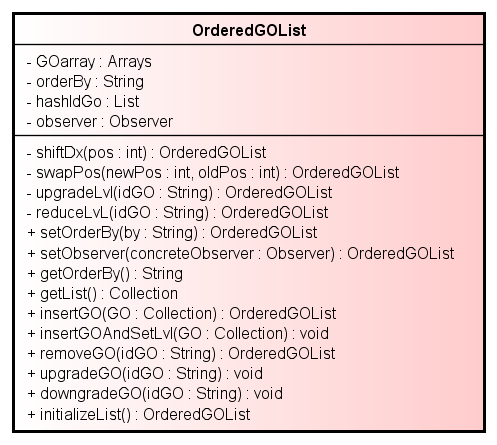
\includegraphics[scale=0.90]{img/diacla/OrderedGOList.png}
\caption{Diagramma della classe premi/client/presentations/lib/OrderedGOList}
\end{center}
\end{figure}


\begin{description}
%-------  descrizione della classe%
\item[Descrizione] \hfill
	Questa classe gestisce una lista ordinata di oggetti grafici da poter essere utilizzata per i frame e l'infografica di una presentazione.
	
	
%-------  lista delle classi associate%	
\item[Dipendenze] \hfill
	\begin{itemize}
		\item \textbf{premi/client/editor/lib/Observer}: per l'invio di segnali che avvertono gli altri componenti delle modifiche apportate agli oggetti grafici
	\end{itemize}
	
	
%-------  lista degli Attributi%	
\item[Attributi] \hfill
	\begin{description}
		\item[\textbf{- GOarray : Array			}] \hfill
			Array di oggetti grafici che compongono la lista ordinata
		\item[\textbf{- orderBy : String			}] \hfill
			Indica il nome dell'attributo che è stato scelto per ordinare gli oggetti grafici
		\item[\textbf{- hashIdGo : List			}] \hfill
			Oggetto Hash$_G$ Javascript$_G$ che contiene una lista degli id degli oggetti grafici presenti nell'array, associati alla loro posizione all'interno dell'array
		\item[\textbf{- observer : Observer			}] \hfill
			Contiene una lista di segnali, ognuno dei quali è associato ad uno specifico oggetto grafico.
	\end{description}
	
	
%-------  lista dei metodi%	
\item[Metodi] \hfill

	% -- inizio metodo -- %
	\begin{description}
		\item[\textbf{\color{blue}- shiftDx(pos : int) : OrderedGOList			}] \hfill
			Sposta l'oggetto grafico presente nella posizione ricevuta nella posizione successiva dell'array. Restituisce un riferimento al \textit{this} per chiamate multiple ai metodi della classe
			
		\begin{description}
			% -- lista argomenti del metodo -- %
			\item[Argomenti] \hfill
				\begin{itemize}
				
					\item \textbf{pos : int			} \hfill
					Posizione dell'oggetto da spostare
					
				\end{itemize}
		\end{description}
	\end{description}
	% -- fine metodo -- %
	
	% -- inizio metodo -- %
	\begin{description}
		\item[\textbf{\color{blue}- swapPos(newPos : int, oldPos : int) : OrderedGOList			}] \hfill
			Scambia di posizione un oggetto grafico. Restituisce un riferimento al \textit{this} per chiamate multiple ai metodi della classe
			
		\begin{description}
			% -- lista argomenti del metodo -- %
			\item[Argomenti] \hfill
				\begin{itemize}
				
					\item \textbf{newPos : int			} \hfill
					La nuova posizione in cui spostare l'oggetto grafico
					\item \textbf{oldPos : int			} \hfill
					La posizione in cui si trova l'oggetto grafico prima dell'esecuzione del metodo
					
				\end{itemize}
		\end{description}
	\end{description}
	% -- fine metodo -- %			
	
	% -- inizio metodo -- %
	\begin{description}
		\item[\textbf{\color{blue}- upgradeLvl(idGO : String) : OrderedGOList			}] \hfill
			Incrementa il livello di visibilità dell'oggetto grafico associato al codice identificativo ricevuto. Restituisce un riferimento al \textit{this} per chiamate multiple ai metodi della classe
			
		\begin{description}
			% -- lista argomenti del metodo -- %
			\item[Argomenti] \hfill
				\begin{itemize}
				
					\item \textbf{idGO : String			} \hfill
					Il codice identificativo dell'oggetto grafico da modificare
					
				\end{itemize}
		\end{description}
	\end{description}
	% -- fine metodo -- %		
	
	% -- inizio metodo -- %
	\begin{description}
		\item[\textbf{\color{blue}- reduceLvl(idGO : String) : OrderedGOList			}] \hfill
			Riduce il livello di visibilità dell'oggetto grafico associato al codice identificativo ricevuto. Restituisce un riferimento al \textit{this} per chiamate multiple ai metodi della classe
			
		\begin{description}
			% -- lista argomenti del metodo -- %
			\item[Argomenti] \hfill
				\begin{itemize}
				
					\item \textbf{idGO : String			} \hfill
					Il codice identificativo dell'oggetto grafico da modificare
					
				\end{itemize}
		\end{description}
	\end{description}
	% -- fine metodo -- %		
	
	% -- inizio metodo -- %
	\begin{description}
		\item[\textbf{\color{blue}+ setOrderBy(by : String) : OrderedGOList			}] \hfill
			Cambia l'attributo con il quale la classe ordina gli oggetti grafici. Restituisce un riferimento al \textit{this} per chiamate multiple ai metodi della classe
			
		\begin{description}
			% -- lista argomenti del metodo -- %
			\item[Argomenti] \hfill
				\begin{itemize}
				
					\item \textbf{by : String			} \hfill
					Il nome dell'attributo con il quale si intende stabilire l'ordine degli oggetti grafici
					
				\end{itemize}
		\end{description}
	\end{description}
	% -- fine metodo -- %	
	
	% -- inizio metodo -- %
	\begin{description}
		\item[\textbf{\color{blue}+ setObserver(concreteObserver : Observer) : OrderedGOList			}] \hfill
			Imposta l'Observer della classe. Restituisce un riferimento al \textit{this} per chiamate multiple ai metodi della classe
			
		\begin{description}
			% -- lista argomenti del metodo -- %
			\item[Argomenti] \hfill
				\begin{itemize}
				
					\item \textbf{concreteObserver : Observer			} \hfill
					L'oggetto Observer da associare alla classe
					
				\end{itemize}
		\end{description}
	\end{description}
	% -- fine metodo -- %	
	
	% -- inizio metodo -- %
	\begin{description}
		\item[\textbf{\color{blue}+ getOrderBy() : String			}] \hfill
			Restituisce il nome dell'attributo col quale si sta effettuando l'ordinamento degli oggetti grafici

	\end{description}
	% -- fine metodo -- %	
	
	% -- inizio metodo -- %
	\begin{description}
		\item[\textbf{\color{blue}+ getList() : Collection			}] \hfill
			Restituisce l'array degli oggetti grafici inseriti finora all'iterno della lista.

	\end{description}
	% -- fine metodo -- %	
	
	% -- inizio metodo -- %
	\begin{description}
		\item[\textbf{\color{blue}+ insertGO(GO : Collection) : OrderedGOList			}] \hfill
			Inserisce un oggetto grafico convertito precedentemente in formato JSON$_G$ all'interno della lista. Restituisce un riferimento al \textit{this} per chiamate multiple ai metodi della classe
			
		\begin{description}
			% -- lista argomenti del metodo -- %
			\item[Argomenti] \hfill
				\begin{itemize}
				
					\item \textbf{GO : Collection			} \hfill
					L'oggetto grafico da inserire nella lista, già convertito in formato JSON
					
				\end{itemize}
		\end{description}
	\end{description}
	% -- fine metodo -- %	
	
	% -- inizio metodo -- %
	\begin{description}
		\item[\textbf{\color{blue}+ insertGOAndSetLvl(GO : Collection) : void			}] \hfill
			Inserisce un oggetto grafico convertito precedentemente in formato JSON$_G$ alla fine della lista, e tramite l'Observer invia un segnale di cambio livello dell'oggetto
			
		\begin{description}
			% -- lista argomenti del metodo -- %
			\item[Argomenti] \hfill
				\begin{itemize}
				
					\item \textbf{GO : Collection			} \hfill
					L'oggetto grafico da inserire nella lista, già convertito in formato JSON
					
				\end{itemize}
		\end{description}
	\end{description}
	% -- fine metodo -- %	
	
	% -- inizio metodo -- %
	\begin{description}
		\item[\textbf{\color{blue}+ removeGO(idGO : String) : OrderedGOList			}] \hfill
			Rimuove un oggetto grafico dalla lista. Restituisce un riferimento al \textit{this} per chiamate multiple ai metodi della classe 
			
		\begin{description}
			% -- lista argomenti del metodo -- %
			\item[Argomenti] \hfill
				\begin{itemize}
				
					\item \textbf{idGO : String			} \hfill
					Il codice identificativo dell'oggetto grafico da rimuovere dalla lista
					
				\end{itemize}
		\end{description}
	\end{description}
	% -- fine metodo -- %	
	
	% -- inizio metodo -- %
	\begin{description}
		\item[\textbf{\color{blue}+ upgradeGO(idGO : String) : void			}] \hfill
			Incrementa di posizione un oggetto grafico nella lista
			
		\begin{description}
			% -- lista argomenti del metodo -- %
			\item[Argomenti] \hfill
				\begin{itemize}
				
					\item \textbf{idGO : String			} \hfill
					Il codice identificativo dell'oggetto grafico da incrementare di posizione
					
				\end{itemize}
				
			% -- note aggiuntive sul metodo -- %
			\item[Note] \hfill
			\begin{itemize}
					\item Sfrutta il metodo privato \textit{swapPos} per li spostamento dell'oggetto grafico
					
			\end{itemize}
		\end{description}
	\end{description}
	% -- fine metodo -- %	
	
	% -- inizio metodo -- %
	\begin{description}
		\item[\textbf{\color{blue}+ downgradeGO(idGO : String) : void			}] \hfill
			Decrementa di posizione un oggetto grafico nella lista
			
		\begin{description}
			% -- lista argomenti del metodo -- %
			\item[Argomenti] \hfill
				\begin{itemize}
				
					\item \textbf{idGO : String			} \hfill
					Il codice identificativo dell'oggetto grafico da decrementare di posizione
					
				\end{itemize}
				
			% -- note aggiuntive sul metodo -- %
			\item[Note] \hfill
			\begin{itemize}
					\item Sfrutta il metodo privato \textit{swapPos} per li spostamento dell'oggetto grafico
					
			\end{itemize}
		\end{description}
	\end{description}
	% -- fine metodo -- %	
	
	% -- inizio metodo -- %
	\begin{description}
		\item[\textbf{\color{blue}+ initializeList() : OrderedGOList			}] \hfill
			Inizializza la lista svuotando \textit{GOarray} \textit{e hashIdGO}. Restituisce un riferimento al \textit{this} per chiamate multiple ai metodi della classe 
			
	\end{description}
	% -- fine metodo -- %
	
		
	

\end{description}






























%-------  diagramma della classe%
\subsubsection{premi/client/presentation/lib/Trail}
\begin{figure}[H]
\begin{center}
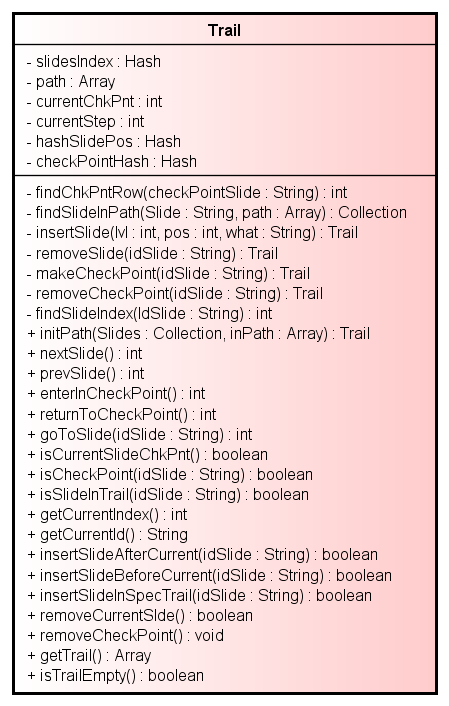
\includegraphics[scale=0.55]{img/diacla/Trail.png}
\caption{Diagramma della classe premi/client/presentation/lib/Trail}
\end{center}
\end{figure}


\begin{description}
%-------  descrizione della classe%
\item[Descrizione] \hfill
	Trail modella un percorso di presentazione, attraverso una lista delle slide contenute al suo interno, e una matrice che rappresenta la struttura del percorso e segnala la presenza di percorsi di specializzazione.
	
	

	
	
%-------  lista degli Attributi%	
\item[Attributi] \hfill
	\begin{description}
		\item[\textbf{- slidesIndex : Hash			}] \hfill
			Lista di tutte le slide contenute all'interno della presentazione create dall'utente. Contiene quindi anche quelle non aggiunte al percorso. È una lista di valori \{ \texttt{id\_{}slide} : \texttt{posizione nell'array di slide} \}
		\item[\textbf{- path : Array			}] \hfill
			Matrice rettangolare che rappresenta il percorso di specializzazione. Contiene i codici identificativi delle slide presenti nel percorso; se non esistono percorsi di specializzazione la matrice sarà composta da una sola riga e tante colonne quante sono le slide presenti al suo interno, la prima collocata nella posizione [0][0]. Ogni riga aggiuntiva indicherà quindi un percorso di specializzazione, che parte dalla slide il cui codice identificativo è inserito nella posizione [riga][0]
			\item[\textbf{- currentChkPnt : int			}] \hfill
			Il checkpoint nel quale l'utente sta lavorando
			\item[\textbf{- currentStep : int			}] \hfill
			Il punto del percorso di specializzazione nel quale l'utente sta lavorando
			\item[\textbf{- hashSlidePos : Hash			}] \hfill
			Lista di codici identificativi delle slide di cui è composto il percorso di presentazione. Sono associati a due integer: \textit{row} indica la riga in cui si trova la slide all'interno della matrice path, mentre \textit{col} indica la colonna
			\item[\textbf{- checkPointHash : Hash		}] \hfill
			Lista delle slide che fungono da checkpoint. È una lista di valori  \{ \texttt{id\_{}slide} : \texttt{riga nella matrice del percorso} \}
	\end{description}
	
	
%-------  lista dei metodi%	
\item[Metodi] \hfill

	% -- inizio metodo -- %
	\begin{description}
		\item[\textbf{\color{blue}- findChkPntRow(checkPointSlide : String) : int			}] \hfill
			Trova la posizione corrispondente della slide che funge da checkpoint all'interno della matrice di presentazione.
			
		\begin{description}
			% -- lista argomenti del metodo -- %
			\item[Argomenti] \hfill
				\begin{itemize}
				
					\item \textbf{checkPointSlide : String		} \hfill
					Codice identificativo della slide
					
				\end{itemize}
			% -- note aggiuntive sul metodo -- %
			\item[Note] \hfill
			\begin{itemize}
					\item Utilizza checkPointHash per restituire il valore. Non è quindi necessario consultare la matrice path
					\item Se la slide non è stata trovata, e non è quindi un checkpoint, restituisce \texttt{-1}
			\end{itemize}
		\end{description}
	\end{description}
	% -- fine metodo -- %		
	
	% -- inizio metodo -- %
	\begin{description}
		\item[\textbf{\color{blue}- findSlideInPath(Slide : String, path : Array) : Collection			}] \hfill
			Trova le coordinate della slide all'interno di una matrice di codici identificativi. Restituisce un hash composto da: \texttt{row}: riga in cui si trova la slide, \texttt{col}: colonna in cui si trova la slide, \texttt{chkRow}: riga in cui si trova la slide se funge anche da checkpoint
			
		\begin{description}
			% -- lista argomenti del metodo -- %
			\item[Argomenti] \hfill
				\begin{itemize}
				
					\item \textbf{Slide : String		} \hfill
					Codice identificativo della slide
					\item \textbf{path : Array		} \hfill
					La matrice in cui cercare la slide
					
				\end{itemize}
			% -- note aggiuntive sul metodo -- %
			\item[Note] \hfill
			\begin{itemize}
					\item row, col, chkRow vanno inizializzati a \texttt{-1} e restituiti con questo valore se la slide non viene trovata
			\end{itemize}
		\end{description}
	\end{description}
	% -- fine metodo -- %	
	
	% -- inizio metodo -- %
	\begin{description}
		\item[\textbf{\color{blue}- insertSlide(lvl : int, pos : int, what : String) : Trail			}] \hfill
			Inserisce il codice identificativo della slide in path, nella posizione indicata dalle coordinate inviate. Restituisce un riferimento al this per consentire chiamate consecutive ai metodi della classe
			
		\begin{description}
			% -- lista argomenti del metodo -- %
			\item[Argomenti] \hfill
				\begin{itemize}
				
					\item \textbf{lvl : int		} \hfill
					Indica la riga in cui si intende inserire la slide
					\item \textbf{pos : int		} \hfill
					Indica la colonna in cui si intende inserire la slide
					\item \textbf{what : String		} \hfill
					È il codice identificativo della slide 
					
				\end{itemize}
			
		\end{description}
	\end{description}
	% -- fine metodo -- %	
	
	% -- inizio metodo -- %
	\begin{description}
		\item[\textbf{\color{blue}- removeSlide(idSlide : String) : Trail			}] \hfill
			Rimuove una slide dal percorso di presentazione. Restituisce un riferimento al this per consentire chiamate consecutive ai metodi della classe
			
		\begin{description}
			% -- lista argomenti del metodo -- %
			\item[Argomenti] \hfill
				\begin{itemize}
					\item \textbf{idSlide : String		} \hfill
					È il codice identificativo della slide 
					
				\end{itemize}
			% -- note aggiuntive sul metodo -- %
			\item[Note] \hfill	
				\begin{itemize}
					\item se la slide da rimuovere è quella nella posizione [0][0], allora l'intero percorso andrà rimosso e hashSlidePos e checkPointHash azzerati
					\item la slide va rimossa da hashSlidePos, e da checkPointHash se fungeva da checkpoint (come vanno rimosse anche le slide incluse nel suo percorso di specializzazione, e se anche qualcuna di queste slide fungeva da checkpoint andranno rimosse ricorsivamente anche le altre slide che dipendevano da essa, etc)
				\end{itemize}
		\end{description}
	\end{description}
	% -- fine metodo -- %	
	
	% -- inizio metodo -- %
	\begin{description}
		\item[\textbf{\color{blue}- makeCheckPoint(idSlide : String) : Trail			}] \hfill
			Imposta la slide come checkpoint. Restituisce un riferimento al this per consentire chiamate consecutive ai metodi della classe
			
		\begin{description}
			% -- lista argomenti del metodo -- %
			\item[Argomenti] \hfill
				\begin{itemize}
				
					\item \textbf{idSlide : String		} \hfill
					È il codice identificativo della slide 
					
				\end{itemize}
			
		\end{description}
	\end{description}
	% -- fine metodo -- %
	
	% -- inizio metodo -- %
	\begin{description}
		\item[\textbf{\color{blue}- removeCheckPoint(idSlide : String) : Trail			}] \hfill
			Rimuove il percorso di specializzazione associato alla slide. Restituisce un riferimento al this per consentire chiamate consecutive ai metodi della classe
			
		\begin{description}
			% -- lista argomenti del metodo -- %
			\item[Argomenti] \hfill
				\begin{itemize}
				
					\item \textbf{idSlide : String		} \hfill
					È il codice identificativo della slide 
					
				\end{itemize}
			
		\end{description}
	\end{description}
	% -- fine metodo -- %
	
	% -- inizio metodo -- %
	\begin{description}
		\item[\textbf{\color{blue}- findSlideIndex(IdSlide : String) : int			}] \hfill
			Restituisce la posizione della slide all'interno della lista di tutte le slide create dall'utente nella presentazione in cui sta lavorando.
			
		\begin{description}
			% -- lista argomenti del metodo -- %
			\item[Argomenti] \hfill
				\begin{itemize}
				
					\item \textbf{idSlide : String		} \hfill
					È il codice identificativo della slide 
					
				\end{itemize}
			
		\end{description}
	\end{description}
	% -- fine metodo -- %
	
	% -- inizio metodo -- %
	\begin{description}
		\item[\textbf{\color{blue}+ initPath(Slides : Collection, inPath : Array) : Trail			}] \hfill
			Data una lista di slides ed una matrice rettangolare, inizializza i tre hash slidesIndex, hashSlidePos e checkPointHash.  Restituisce un riferimento al this per consentire chiamate consecutive ai metodi della classe
			
		\begin{description}
			% -- lista argomenti del metodo -- %
			\item[Argomenti] \hfill
				\begin{itemize}
				
					\item \textbf{Slides : Collection		} \hfill
					È una collezione di tutte le slides create dall'utente nella presentazione in cui sta lavorando
					\item \textbf{inPath :  Array		} \hfill
					È la matrice rettangolare che rappresenta il percorso della presentazione
					
				\end{itemize}
			
		\end{description}
	\end{description}
	% -- fine metodo -- %
	
	% -- inizio metodo -- %
	\begin{description}
		\item[\textbf{\color{blue}+ nextSlide() : int			}] \hfill
			Restituisce la posizione (all'interno della lista di tutte le slides create dall'utente nella presentazione corrente) della prossima slide rispetto alla posizione in cui l'utente si trova nel percorso che sta visualizzando.
			
	\end{description}
	% -- fine metodo -- %
	
	% -- inizio metodo -- %
	\begin{description}
		\item[\textbf{\color{blue}+ prevSlide() : int			}] \hfill
			Restituisce la posizione (all'interno della lista di tutte le slides create dall'utente nella presentazione corrente) della slide precedente rispetto alla posizione in cui l'utente si trova nel percorso che sta visualizzando.
			
	\end{description}
	% -- fine metodo -- %
	
	
	% -- inizio metodo -- %
	\begin{description}
		\item[\textbf{\color{blue}+ enterInCheckPoint() : int			}] \hfill
			Restituisce la riga in cui si trova il percorso di specializzazione della slide che l'utente sta visualizzando, solo se la slide funge da checkpoint
			
		\begin{description}
			
			% -- note aggiuntive sul metodo -- %
			\item[Note] \hfill	
				\begin{itemize}
					\item restituisce -1 se la slide non è un checkpoint o se è la slide nella posizione [0][0]
				\end{itemize}
		\end{description}
			
	\end{description}
	% -- fine metodo -- %
	
	% -- inizio metodo -- %
	\begin{description}
		\item[\textbf{\color{blue}+ returnToCheckPoint() : int			}] \hfill
			Ritorna al percorso in cui l'utente si trovava prima di di accedere ad un percorso di specializzazione
			
		\begin{description}
			
			% -- note aggiuntive sul metodo -- %
			\item[Note] \hfill	
				\begin{itemize}
					\item restituisce -1 se l'utente non si trova in un percorso di specializzazione
				\end{itemize}
		\end{description}
			
	\end{description}
	% -- fine metodo -- %
	
	% -- inizio metodo -- %
	\begin{description}
		\item[\textbf{\color{blue}+ goToSlide(idSlide : String) : int			}] \hfill
			Sposta la visualizzazione sulla slide ricevuta, se presente all'interno del percorso, e restituisce la posizione della slide all'interno di slidesIndex
			
		\begin{description}
			% -- lista argomenti del metodo -- %
			\item[Argomenti] \hfill
				\begin{itemize}
				
					\item \textbf{idSlide : String	} \hfill
					È il codice identificativo della slide
					
				\end{itemize}
			
		\end{description}
	\end{description}
	% -- fine metodo -- %
	
	% -- inizio metodo -- %
	\begin{description}
		\item[\textbf{\color{blue}+ isCurrentSlideChkPnt() : boolean			}] \hfill
			Restituisce \textit{true} se la slide in cui l'utente si trova è un checkpoint, \textit{false} altrimenti
			
	\end{description}
	% -- fine metodo -- %
	
	% -- inizio metodo -- %
	\begin{description}
		\item[\textbf{\color{blue}+ isCheckPoint(idSlide : String) : boolean			}] \hfill
			Restituisce \textit{true} se la slide corrispondente al codice identificativo rievuto è un checkpoint, \textit{false} altrimenti
			
		\begin{description}
			% -- lista argomenti del metodo -- %
			\item[Argomenti] \hfill
				\begin{itemize}
				
					\item \textbf{idSlide : String	} \hfill
					È il codice identificativo della slide
					
				\end{itemize}
			
		\end{description}
			
	\end{description}
	% -- fine metodo -- %
	
	% -- inizio metodo -- %
	\begin{description}
		\item[\textbf{\color{blue}+ isSlideInTrail(idSlide : String) : boolean			}] \hfill
			Restituisce \textit{true} se la slide corrispondente al codice identificativo rievuto è presente all'interno del percorso, \textit{false} altrimenti
			
		\begin{description}
			% -- lista argomenti del metodo -- %
			\item[Argomenti] \hfill
				\begin{itemize}
				
					\item \textbf{idSlide : String	} \hfill
					È il codice identificativo della slide
					
				\end{itemize}
			
		\end{description}
			
	\end{description}
	% -- fine metodo -- %
	
	% -- inizio metodo -- %
	\begin{description}
		\item[\textbf{\color{blue}+ getCurrentIndex() : int			}] \hfill
			Restituisce la posizione in slidesIndex della slide attualmente selezionata
			
	\end{description}
	% -- fine metodo -- %
	
	% -- inizio metodo -- %
	\begin{description}
		\item[\textbf{\color{blue}+ getCurrentId() : String			}] \hfill
			Restituisce il codice identificativo della slide attualmente selezionata
			
	\end{description}
	% -- fine metodo -- %
	
	% -- inizio metodo -- %
	\begin{description}
		\item[\textbf{\color{blue}+ insertSlideAfterCurrent(idSlide : String) : boolean			}] \hfill
			Inserisce la slide ricevuta nella posizione successiva a quella attualmente selezionata. Restituisce \textit{true} se l'operazione ha avuto successo, \textit{false} altrimenti
			
		\begin{description}
			% -- lista argomenti del metodo -- %
			\item[Argomenti] \hfill
				\begin{itemize}
				
					\item \textbf{idSlide : String	} \hfill
					È il codice identificativo della slide
					
				\end{itemize}
			
		\end{description}
			
	\end{description}
	% -- fine metodo -- %
	
	% -- inizio metodo -- %
	\begin{description}
		\item[\textbf{\color{blue}+ insertSlideAfterCurrent(idSlide : String) : boolean			}] \hfill
			Inserisce la slide ricevuta nella posizione precedente a quella attualmente selezionata. Restituisce \textit{true} se l'operazione ha avuto successo, \textit{false} altrimenti
			
		\begin{description}
			% -- lista argomenti del metodo -- %
			\item[Argomenti] \hfill
				\begin{itemize}
				
					\item \textbf{idSlide : String	} \hfill
					È il codice identificativo della slide
					
				\end{itemize}
			
		\end{description}
			
	\end{description}
	% -- fine metodo -- %
	
	% -- inizio metodo -- %
	\begin{description}
		\item[\textbf{\color{blue}+ insertSlideAfterCurrent(idSlide : String) : boolean			}] \hfill
			Inserisce la slide ricevuta nel percorso di specializzazione correlato alla slide attualmente selezionata. Se la slide non era un checkpoint viene impostata come tale. Restituisce \textit{true} se l'operazione ha avuto successo, \textit{false} altrimenti
			
		\begin{description}
			% -- lista argomenti del metodo -- %
			\item[Argomenti] \hfill
				\begin{itemize}
				
					\item \textbf{idSlide : String	} \hfill
					È il codice identificativo della slide
					
				\end{itemize}
			
		\end{description}
			
	\end{description}
	% -- fine metodo -- %
	
	% -- inizio metodo -- %
	\begin{description}
		\item[\textbf{\color{blue}+ removeCurrentSlde() : boolean			}] \hfill
			Rimuove la slide attualmente selezionata. Restituisce \textit{true} se l'operazione ha avuto successo, \textit{false} altrimenti 
			
	\end{description}
	% -- fine metodo -- %
	
	% -- inizio metodo -- %
	\begin{description}
		\item[\textbf{\color{blue}+ removeCheckPoint() : void			}] \hfill
			Toglie il percorso di specializzazione dalla slide attualmente selezionata, che non sarà più un checkpoint
			
	\end{description}
	% -- fine metodo -- %
	
	% -- inizio metodo -- %
	\begin{description}
		\item[\textbf{\color{blue}+ getTrail() : Array			}] \hfill
			Restituisce l'array path
			
	\end{description}
	% -- fine metodo -- %
	
	% -- inizio metodo -- %
	\begin{description}
		\item[\textbf{\color{blue}+ isTrailEmpty() : Boolean			}] \hfill
			Restituisce \textit{true} se il percorso è vuoto, \textit{false} altrimenti
			
	\end{description}
	% -- fine metodo -- %
	
	

\end{description}

%-------  diagramma della classe%
\subsubsection{premi/client/presentation/lib/signalCtrl}
\begin{figure}[H]
\begin{center}
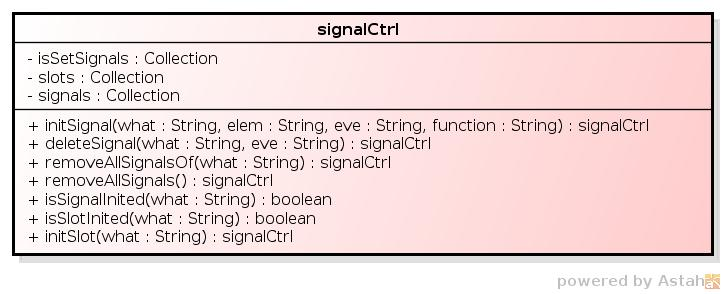
\includegraphics[scale=0.55]{img/diacla/signalCtrl.jpg}
\caption{Diagramma della classe premi/client/presentation/lib/signalCtrl}
\end{center}
\end{figure}


\begin{description}
%-------  descrizione della classe%
\item[Descrizione] \hfill
	Questa classe ha lo scopo di registrare i signal quando un certo slot viene creato in modo tale che facendo un controllo sul relativo controller si eviti di aggiungerne in più.
Inoltre potrà registrare i listner associati a qualche elemento del DOM (di solito il document stesso) in modo tale da rimuovere/aggiungere dinamicamente i listner giusti a seconda dello stato in cui si trova l'applicazione.
	
%-------  lista degli Attributi%	
\item[Attributi] \hfill
	\begin{description}
		\item[\textbf{- isSetSignals : Collection			}] \hfill
			Oggetto JSON che indica per ogni campo che contiene se è presente almeno un Signal. I campi che contiene sono:
			\begin{itemize}
				\item \textit{infographic:} identifica l'oggetto infographic;
				\item \textit{trails:} identifica gli oggetti trail;
				\item \textit{viewer:} identifica gli oggetti viewer.  
			\end{itemize} 
		\item[\textbf{- slots : Collection			}] \hfill
			Oggetto JSON che indica per ogni campo che contiene se è stato creato un certo slots. I campi che contiene sono:
			\begin{itemize}
				\item \textit{infographic:} identifica l'oggetto infographic;
				\item \textit{trails:} identifica gli oggetti trail;
				\item \textit{viewer:} identifica gli oggetti viewer.  
			\end{itemize} 
		\item[\textbf{- signals : Collection			}] \hfill
			Oggetto JSON che indica per ogni campo quali sono i signal presenti:
			\begin{itemize}
				\item \textit{infographic:} identifica i signal dell'oggetto infographic;
				\item \textit{trails:} identifica i signal degli oggetti trail;
				\item \textit{viewer:} identifica i signal degli oggetti viewer.  
			\end{itemize} 
	\end{description}
	
	
%-------  lista dei metodi%	
\item[Metodi] \hfill

	% -- inizio metodo -- %
	\begin{description}
		\item[\textbf{\color{blue}+ initSignal(what : String, elem : String, eve : String, func : String) : signalCtrl			}] \hfill
			inizializza i signal di un oggetto.
			
		\begin{description}
			% -- lista argomenti del metodo -- %
			\item[Argomenti] \hfill
				\begin{itemize}
				
					\item \textbf{what : String			} \hfill
					identifica l'oggetto (infographic, trails, viewer);
					\item \textbf{elem : String			} \hfill
					identifica l'elemento su cui fa riferimento un signal;
					\item \textbf{eve : String			} \hfill
					rappresenta l'evento;
					\item \textbf{func : String			} \hfill
					rappresenta la funzione.
					
				\end{itemize}
		\end{description}
	\end{description}
	% -- fine metodo -- %
	
	% -- inizio metodo -- %
	\begin{description}
		\item[\textbf{\color{blue}+ deleteSignal(what : String, eve : String) : signalCtrl			}] \hfill
			rimuove i signal che si riferiscono ad un certo evento.
			
		\begin{description}
			% -- lista argomenti del metodo -- %
			\item[Argomenti] \hfill
				\begin{itemize}
				
					\item \textbf{what : String			} \hfill
					identifica l'oggetto (infographic, trails, viewer) su cui eliminare i signal;
					\item \textbf{eve : String			} \hfill
					identifica l'evento.
					
				\end{itemize}
		\end{description}
	\end{description}
	% -- fine metodo -- %
	
	% -- inizio metodo -- %
	\begin{description}
		\item[\textbf{\color{blue}+ removeAllSignalOf(what : String) : signalCtrl			}] \hfill
			rimuove tutti i signal di un determinato oggetto.
			
		\begin{description}
			% -- lista argomenti del metodo -- %
			\item[Argomenti] \hfill
				\begin{itemize}
				
					\item \textbf{what : String			} \hfill
					identifica l'oggetto (infographic, trails, viewer);
					
				\end{itemize}
		\end{description}
	\end{description}
	% -- fine metodo -- %
	
	% -- inizio metodo -- %
	\begin{description}
		\item[\textbf{\color{blue}+ removeAllSignals() : signalCtrl		}] \hfill
			rimuove tutti i signal di tutti gli oggetti.
			
	\end{description}
	% -- fine metodo -- %
	
	% -- inizio metodo -- %
	\begin{description}
		\item[\textbf{\color{blue}+ isSignalInited(what : String) : boolean			}] \hfill
			restituisce true se è impostato almeno un signal di un determinato oggetto.
			
		\begin{description}
			% -- lista argomenti del metodo -- %
			\item[Argomenti] \hfill
				\begin{itemize}
				
					\item \textbf{what : String			} \hfill
					identifica l'oggetto (infographic, trails, viewer) su cui controllare i signal;
					
				\end{itemize}
		\end{description}
	\end{description}
	% -- fine metodo -- %
	
	% -- inizio metodo -- %
	\begin{description}
		\item[\textbf{\color{blue}+ initSlot(what : String) : signalCtrl			}] \hfill
			inizializza gli slot di un determinato oggetto.
			
		\begin{description}
			% -- lista argomenti del metodo -- %
			\item[Argomenti] \hfill
				\begin{itemize}
				
					\item \textbf{what : String			} \hfill
					identifica l'oggetto (infographic, trails, viewer);
					
				\end{itemize}
		\end{description}
	\end{description}
	% -- fine metodo -- %
			
	% -- inizio metodo -- %
	\begin{description}
		\item[\textbf{\color{blue}+ isSlotInited(what : String) : boolean			}] \hfill
			restituisce true se è stato inizializzato almeno uno slot su un determinato oggetto.
			
		\begin{description}
			% -- lista argomenti del metodo -- %
			\item[Argomenti] \hfill
				\begin{itemize}
				
					\item \textbf{what : String			} \hfill
					identifica l'oggetto (infographic, trails, viewer) su cui controllare gli slot.
					
				\end{itemize}
		\end{description}
	\end{description}
	% -- fine metodo -- %
	
	% -- inizio metodo -- %
	\begin{description}
		\item[\textbf{\color{blue}+ initSlot(what : String) : signalCtrl			}] \hfill
			inizializza uno slot su un determinato oggetto.
			
		\begin{description}
			% -- lista argomenti del metodo -- %
			\item[Argomenti] \hfill
				\begin{itemize}
				
					\item \textbf{what : String			} \hfill
					identifica l'oggetto (infographic, trails, viewer);
					
				\end{itemize}
		\end{description}
	\end{description}
	% -- fine metodo -- %
				

\end{description}






























